%Design – in design section you should describe your approach to solve the problem. The high level design of your solution and the modules, data structures and algorithms that you use.

\section{Design} 

\subsection{Considered modifications}
Viacero z prezentovaných modifikácií boli aplikované na iné typy neurónových sietí. My sme sa zaoberali aplikáciami na Generec, analyzovali sme ich konvergenciu a aplikovali ich na štandardnej sade úloh. 

\subsubsection{Regression} 

\textit{Regression} means that, after one pass around the loop, instead of setting the activity of a visible unit, $i$, to be equal to its current total input, $x_i(2)$, as determined by 
$$x_j = \sum_i y_iw_{ji} - \theta_j,$$
we set its activity to be 
$$y_i(2) = \lambda y_i(0) + (1-\lambda)x_i(2)$$
where the regression, $\lambda$, is close to 1. Using high regression ensures that the visible units only change state slightly so that when the new visible vector is sent around the loop again on the second pass, it has very similar effects to the first pass \cite{hinton1988learning}.

\subsubsection{Ballard}
Merging several closed loops of recirculation. 

Since the same learning rule is used for both visivle and hidden units, there is no problem in applying it to systems in which some units are the visible units of one module and the hidden units of another \cite{hinton1988learning}. 

We do not have a formal analysis \cite{hinton1988learning}.
%D.H. Ballard Proc. American Association for Artificial Intelligence, Seatle, WA, 1987

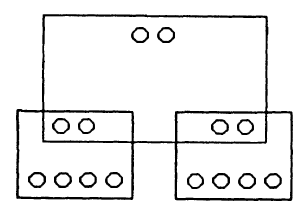
\includegraphics[width=8cm]{img/ballard.png}

\subsubsection{Dropout}
When a large feedforward neural network is trained on a small training set,
it typically performs poorly on held-out test data. This \emph{overfitting} is greatly
reduced by randomly omitting half of the feature detectors on each training
case. This prevents complex co-adaptations in which a feature detector is only
helpful in the context of several other specific feature detectors. Instead, each
neuron learns to detect a feature that is generally helpful for producing the
correct answer given the combinatorially large variety of internal contexts in
which it must operate. Random \emph{dropout} gives big improvements on many
benchmark tasks and sets new records for speech and object recognition.
 \cite{hinton2012improving} (Abstract copied). 
 
 TODO: Read the article. 
 
Conceptually the idea is simple. In each activation phase turn off randomly a half of all hidden neurons. This should restrict coadaptation of neurons. It a desired quality as we want from each unit to represent a different feature. If the units can coadapt then it might occur that more units represent the same feature. 

\subsubsection{Deep architectures} 
TODO  \cite{bengio2009learning}.

